% Created by tikzDevice version 0.12.6 on 2025-12-23 06:15:30
% !TEX encoding = UTF-8 Unicode
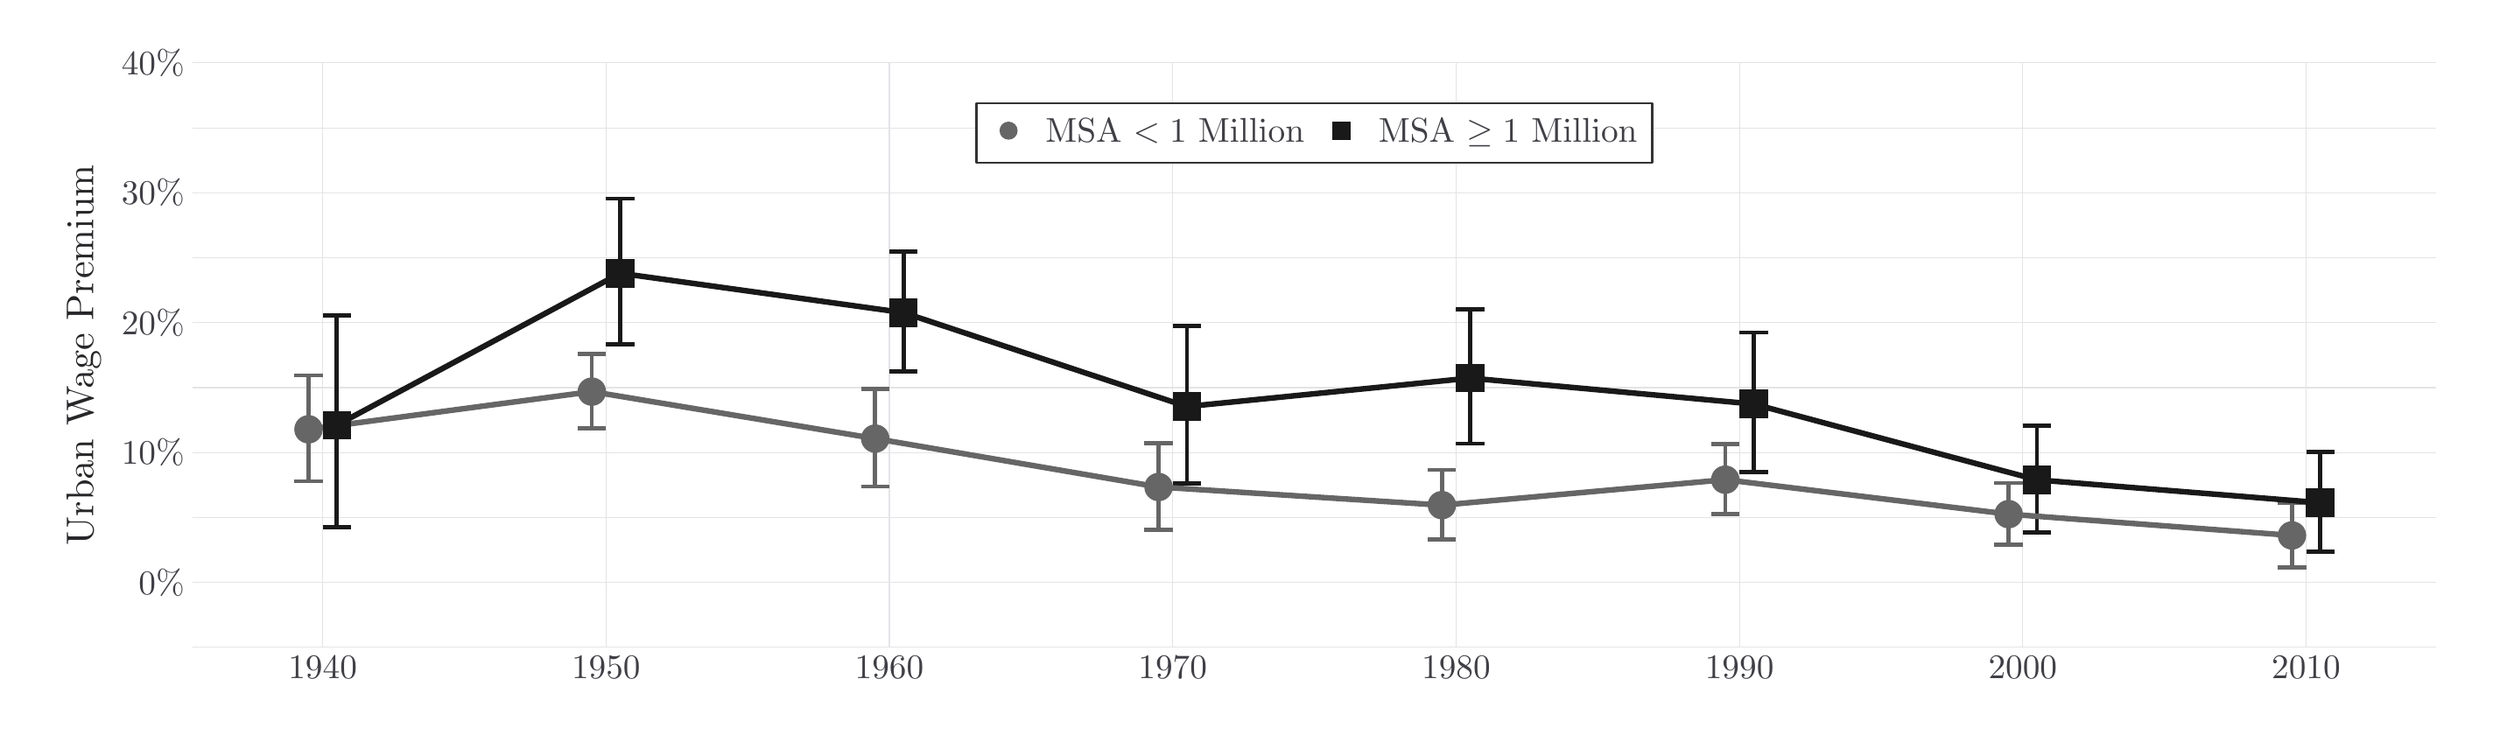
\begin{tikzpicture}[x=1pt,y=1pt]
\definecolor{fillColor}{RGB}{255,255,255}
\path[use as bounding box,fill=fillColor] (0,0) rectangle (1011.78,289.08);
\begin{scope}
\path[clip] (  0.00,  0.00) rectangle (1011.78,289.08);
\definecolor{drawColor}{RGB}{255,255,255}

\path[draw=drawColor,line width= 0.8pt,line join=round,line cap=round,fill=fillColor] (  0.00,  0.00) rectangle (1011.78,289.08);
\end{scope}
\begin{scope}
\path[clip] ( 69.39, 31.76) rectangle (995.78,273.08);
\definecolor{drawColor}{RGB}{255,255,255}
\definecolor{fillColor}{RGB}{255,255,255}

\path[draw=drawColor,line width= 0.8pt,line join=round,line cap=round,fill=fillColor] ( 69.39, 31.76) rectangle (995.78,273.08);
\definecolor{drawColor}{RGB}{228,228,231}

\path[draw=drawColor,line width= 0.4pt,line join=round] ( 69.39, 31.76) --
	(995.78, 31.76);

\path[draw=drawColor,line width= 0.4pt,line join=round] ( 69.39, 85.39) --
	(995.78, 85.39);

\path[draw=drawColor,line width= 0.4pt,line join=round] ( 69.39,139.01) --
	(995.78,139.01);

\path[draw=drawColor,line width= 0.4pt,line join=round] ( 69.39,192.64) --
	(995.78,192.64);

\path[draw=drawColor,line width= 0.4pt,line join=round] ( 69.39,246.27) --
	(995.78,246.27);

\path[draw=drawColor,line width= 0.4pt,line join=round] ( 69.39, 58.57) --
	(995.78, 58.57);

\path[draw=drawColor,line width= 0.4pt,line join=round] ( 69.39,112.20) --
	(995.78,112.20);

\path[draw=drawColor,line width= 0.4pt,line join=round] ( 69.39,165.83) --
	(995.78,165.83);

\path[draw=drawColor,line width= 0.4pt,line join=round] ( 69.39,219.45) --
	(995.78,219.45);

\path[draw=drawColor,line width= 0.4pt,line join=round] ( 69.39,273.08) --
	(995.78,273.08);

\path[draw=drawColor,line width= 0.4pt,line join=round] (123.20, 31.76) --
	(123.20,273.08);

\path[draw=drawColor,line width= 0.4pt,line join=round] (240.17, 31.76) --
	(240.17,273.08);

\path[draw=drawColor,line width= 0.4pt,line join=round] (357.13, 31.76) --
	(357.13,273.08);

\path[draw=drawColor,line width= 0.4pt,line join=round] (474.10, 31.76) --
	(474.10,273.08);

\path[draw=drawColor,line width= 0.4pt,line join=round] (591.07, 31.76) --
	(591.07,273.08);

\path[draw=drawColor,line width= 0.4pt,line join=round] (708.04, 31.76) --
	(708.04,273.08);

\path[draw=drawColor,line width= 0.4pt,line join=round] (825.01, 31.76) --
	(825.01,273.08);

\path[draw=drawColor,line width= 0.4pt,line join=round] (941.97, 31.76) --
	(941.97,273.08);
\definecolor{drawColor}{gray}{0.40}

\path[draw=drawColor,line width= 1.7pt,line join=round] (111.50,144.04) --
	(123.20,144.04);

\path[draw=drawColor,line width= 1.7pt,line join=round] (117.35,144.04) --
	(117.35,100.31);

\path[draw=drawColor,line width= 1.7pt,line join=round] (111.50,100.31) --
	(123.20,100.31);
\definecolor{drawColor}{gray}{0.10}

\path[draw=drawColor,line width= 1.7pt,line join=round] (123.20,168.70) --
	(134.90,168.70);

\path[draw=drawColor,line width= 1.7pt,line join=round] (129.05,168.70) --
	(129.05, 81.48);

\path[draw=drawColor,line width= 1.7pt,line join=round] (123.20, 81.48) --
	(134.90, 81.48);
\definecolor{drawColor}{gray}{0.40}

\path[draw=drawColor,line width= 1.7pt,line join=round] (228.47,152.96) --
	(240.17,152.96);

\path[draw=drawColor,line width= 1.7pt,line join=round] (234.32,152.96) --
	(234.32,122.13);

\path[draw=drawColor,line width= 1.7pt,line join=round] (228.47,122.13) --
	(240.17,122.13);
\definecolor{drawColor}{gray}{0.10}

\path[draw=drawColor,line width= 1.7pt,line join=round] (240.17,217.00) --
	(251.86,217.00);

\path[draw=drawColor,line width= 1.7pt,line join=round] (246.02,217.00) --
	(246.02,156.80);

\path[draw=drawColor,line width= 1.7pt,line join=round] (240.17,156.80) --
	(251.86,156.80);
\definecolor{drawColor}{gray}{0.40}

\path[draw=drawColor,line width= 1.7pt,line join=round] (345.44,138.39) --
	(357.13,138.39);

\path[draw=drawColor,line width= 1.7pt,line join=round] (351.29,138.39) --
	(351.29, 98.20);

\path[draw=drawColor,line width= 1.7pt,line join=round] (345.44, 98.20) --
	(357.13, 98.20);
\definecolor{drawColor}{gray}{0.10}

\path[draw=drawColor,line width= 1.7pt,line join=round] (357.13,195.30) --
	(368.83,195.30);

\path[draw=drawColor,line width= 1.7pt,line join=round] (362.98,195.30) --
	(362.98,145.59);

\path[draw=drawColor,line width= 1.7pt,line join=round] (357.13,145.59) --
	(368.83,145.59);
\definecolor{drawColor}{gray}{0.40}

\path[draw=drawColor,line width= 1.7pt,line join=round] (462.41,116.11) --
	(474.10,116.11);

\path[draw=drawColor,line width= 1.7pt,line join=round] (468.25,116.11) --
	(468.25, 80.37);

\path[draw=drawColor,line width= 1.7pt,line join=round] (462.41, 80.37) --
	(474.10, 80.37);
\definecolor{drawColor}{gray}{0.10}

\path[draw=drawColor,line width= 1.7pt,line join=round] (474.10,164.58) --
	(485.80,164.58);

\path[draw=drawColor,line width= 1.7pt,line join=round] (479.95,164.58) --
	(479.95, 99.51);

\path[draw=drawColor,line width= 1.7pt,line join=round] (474.10, 99.51) --
	(485.80, 99.51);
\definecolor{drawColor}{gray}{0.40}

\path[draw=drawColor,line width= 1.7pt,line join=round] (579.37,105.06) --
	(591.07,105.06);

\path[draw=drawColor,line width= 1.7pt,line join=round] (585.22,105.06) --
	(585.22, 76.24);

\path[draw=drawColor,line width= 1.7pt,line join=round] (579.37, 76.24) --
	(591.07, 76.24);
\definecolor{drawColor}{gray}{0.10}

\path[draw=drawColor,line width= 1.7pt,line join=round] (591.07,171.24) --
	(602.77,171.24);

\path[draw=drawColor,line width= 1.7pt,line join=round] (596.92,171.24) --
	(596.92,115.86);

\path[draw=drawColor,line width= 1.7pt,line join=round] (591.07,115.86) --
	(602.77,115.86);
\definecolor{drawColor}{gray}{0.40}

\path[draw=drawColor,line width= 1.7pt,line join=round] (696.34,115.62) --
	(708.04,115.62);

\path[draw=drawColor,line width= 1.7pt,line join=round] (702.19,115.62) --
	(702.19, 86.70);

\path[draw=drawColor,line width= 1.7pt,line join=round] (696.34, 86.70) --
	(708.04, 86.70);
\definecolor{drawColor}{gray}{0.10}

\path[draw=drawColor,line width= 1.7pt,line join=round] (708.04,161.78) --
	(719.74,161.78);

\path[draw=drawColor,line width= 1.7pt,line join=round] (713.89,161.78) --
	(713.89,104.05);

\path[draw=drawColor,line width= 1.7pt,line join=round] (708.04,104.05) --
	(719.74,104.05);
\definecolor{drawColor}{gray}{0.40}

\path[draw=drawColor,line width= 1.7pt,line join=round] (813.31, 99.57) --
	(825.01, 99.57);

\path[draw=drawColor,line width= 1.7pt,line join=round] (819.16, 99.57) --
	(819.16, 74.22);

\path[draw=drawColor,line width= 1.7pt,line join=round] (813.31, 74.22) --
	(825.01, 74.22);
\definecolor{drawColor}{gray}{0.10}

\path[draw=drawColor,line width= 1.7pt,line join=round] (825.01,123.38) --
	(836.70,123.38);

\path[draw=drawColor,line width= 1.7pt,line join=round] (830.86,123.38) --
	(830.86, 79.28);

\path[draw=drawColor,line width= 1.7pt,line join=round] (825.01, 79.28) --
	(836.70, 79.28);
\definecolor{drawColor}{gray}{0.40}

\path[draw=drawColor,line width= 1.7pt,line join=round] (930.28, 91.50) --
	(941.97, 91.50);

\path[draw=drawColor,line width= 1.7pt,line join=round] (936.13, 91.50) --
	(936.13, 64.74);

\path[draw=drawColor,line width= 1.7pt,line join=round] (930.28, 64.74) --
	(941.97, 64.74);
\definecolor{drawColor}{gray}{0.10}

\path[draw=drawColor,line width= 1.7pt,line join=round] (941.97,112.47) --
	(953.67,112.47);

\path[draw=drawColor,line width= 1.7pt,line join=round] (947.82,112.47) --
	(947.82, 71.22);

\path[draw=drawColor,line width= 1.7pt,line join=round] (941.97, 71.22) --
	(953.67, 71.22);
\definecolor{drawColor}{gray}{0.40}

\path[draw=drawColor,line width= 2.3pt,line join=round] (117.35,121.78) --
	(234.32,137.35) --
	(351.29,117.95) --
	(468.25, 97.96) --
	(585.22, 90.47) --
	(702.19,100.98) --
	(819.16, 86.75) --
	(936.13, 77.96);
\definecolor{drawColor}{gray}{0.10}

\path[draw=drawColor,line width= 2.3pt,line join=round] (129.05,123.51) --
	(246.02,186.22) --
	(362.98,169.97) --
	(479.95,131.18) --
	(596.92,142.93) --
	(713.89,132.23) --
	(830.86,100.91) --
	(947.82, 91.47);
\definecolor{fillColor}{gray}{0.40}

\path[fill=fillColor] (117.35,121.78) circle (  5.87);
\definecolor{fillColor}{gray}{0.10}

\path[fill=fillColor] (123.17,117.64) --
	(134.92,117.64) --
	(134.92,129.38) --
	(123.17,129.38) --
	cycle;
\definecolor{fillColor}{gray}{0.40}

\path[fill=fillColor] (234.32,137.35) circle (  5.87);
\definecolor{fillColor}{gray}{0.10}

\path[fill=fillColor] (240.14,180.35) --
	(251.89,180.35) --
	(251.89,192.09) --
	(240.14,192.09) --
	cycle;
\definecolor{fillColor}{gray}{0.40}

\path[fill=fillColor] (351.29,117.95) circle (  5.87);
\definecolor{fillColor}{gray}{0.10}

\path[fill=fillColor] (357.11,164.10) --
	(368.86,164.10) --
	(368.86,175.84) --
	(357.11,175.84) --
	cycle;
\definecolor{fillColor}{gray}{0.40}

\path[fill=fillColor] (468.25, 97.96) circle (  5.87);
\definecolor{fillColor}{gray}{0.10}

\path[fill=fillColor] (474.08,125.30) --
	(485.82,125.30) --
	(485.82,137.05) --
	(474.08,137.05) --
	cycle;
\definecolor{fillColor}{gray}{0.40}

\path[fill=fillColor] (585.22, 90.47) circle (  5.87);
\definecolor{fillColor}{gray}{0.10}

\path[fill=fillColor] (591.05,137.06) --
	(602.79,137.06) --
	(602.79,148.80) --
	(591.05,148.80) --
	cycle;
\definecolor{fillColor}{gray}{0.40}

\path[fill=fillColor] (702.19,100.98) circle (  5.87);
\definecolor{fillColor}{gray}{0.10}

\path[fill=fillColor] (708.01,126.36) --
	(719.76,126.36) --
	(719.76,138.10) --
	(708.01,138.10) --
	cycle;
\definecolor{fillColor}{gray}{0.40}

\path[fill=fillColor] (819.16, 86.75) circle (  5.87);
\definecolor{fillColor}{gray}{0.10}

\path[fill=fillColor] (824.98, 95.04) --
	(836.73, 95.04) --
	(836.73,106.78) --
	(824.98,106.78) --
	cycle;
\definecolor{fillColor}{gray}{0.40}

\path[fill=fillColor] (936.13, 77.96) circle (  5.87);
\definecolor{fillColor}{gray}{0.10}

\path[fill=fillColor] (941.95, 85.60) --
	(953.70, 85.60) --
	(953.70, 97.34) --
	(941.95, 97.34) --
	cycle;
\end{scope}
\begin{scope}
\path[clip] (  0.00,  0.00) rectangle (1011.78,289.08);
\definecolor{drawColor}{RGB}{63,63,70}

\node[text=drawColor,anchor=base east,inner sep=0pt, outer sep=0pt, scale=  1.42] at ( 66.19, 53.67) {0\%};

\node[text=drawColor,anchor=base east,inner sep=0pt, outer sep=0pt, scale=  1.42] at ( 66.19,107.30) {10\%};

\node[text=drawColor,anchor=base east,inner sep=0pt, outer sep=0pt, scale=  1.42] at ( 66.19,160.93) {20\%};

\node[text=drawColor,anchor=base east,inner sep=0pt, outer sep=0pt, scale=  1.42] at ( 66.19,214.56) {30\%};

\node[text=drawColor,anchor=base east,inner sep=0pt, outer sep=0pt, scale=  1.42] at ( 66.19,268.18) {40\%};
\end{scope}
\begin{scope}
\path[clip] (  0.00,  0.00) rectangle (1011.78,289.08);
\definecolor{drawColor}{RGB}{63,63,70}

\node[text=drawColor,anchor=base,inner sep=0pt, outer sep=0pt, scale=  1.42] at (123.20, 18.76) {1940};

\node[text=drawColor,anchor=base,inner sep=0pt, outer sep=0pt, scale=  1.42] at (240.17, 18.76) {1950};

\node[text=drawColor,anchor=base,inner sep=0pt, outer sep=0pt, scale=  1.42] at (357.13, 18.76) {1960};

\node[text=drawColor,anchor=base,inner sep=0pt, outer sep=0pt, scale=  1.42] at (474.10, 18.76) {1970};

\node[text=drawColor,anchor=base,inner sep=0pt, outer sep=0pt, scale=  1.42] at (591.07, 18.76) {1980};

\node[text=drawColor,anchor=base,inner sep=0pt, outer sep=0pt, scale=  1.42] at (708.04, 18.76) {1990};

\node[text=drawColor,anchor=base,inner sep=0pt, outer sep=0pt, scale=  1.42] at (825.01, 18.76) {2000};

\node[text=drawColor,anchor=base,inner sep=0pt, outer sep=0pt, scale=  1.42] at (941.97, 18.76) {2010};
\end{scope}
\begin{scope}
\path[clip] (  0.00,  0.00) rectangle (1011.78,289.08);
\definecolor{drawColor}{RGB}{39,39,42}

\node[text=drawColor,rotate= 90.00,anchor=base,inner sep=0pt, outer sep=0pt, scale=  1.60] at ( 28.57,152.42) {Urban Wage Premium};
\end{scope}
\begin{scope}
\path[clip] (  0.00,  0.00) rectangle (1011.78,289.08);
\definecolor{drawColor}{gray}{0.20}
\definecolor{fillColor}{RGB}{255,255,255}

\path[draw=drawColor,line width= 0.8pt,line join=round,line cap=round,fill=fillColor] (393.11,231.89) rectangle (672.06,256.35);
\end{scope}
\begin{scope}
\path[clip] (  0.00,  0.00) rectangle (1011.78,289.08);
\definecolor{drawColor}{RGB}{255,255,255}
\definecolor{fillColor}{RGB}{255,255,255}

\path[draw=drawColor,line width= 0.8pt,line join=round,line cap=round,fill=fillColor] (399.11,237.89) rectangle (413.56,252.35);

\path[] (400.55,245.12) -- (412.12,245.12);

\path[] (400.55,245.12) -- (412.12,245.12);
\definecolor{fillColor}{gray}{0.40}

\path[fill=fillColor] (406.34,245.12) circle (  3.73);
\end{scope}
\begin{scope}
\path[clip] (  0.00,  0.00) rectangle (1011.78,289.08);
\definecolor{drawColor}{RGB}{255,255,255}
\definecolor{fillColor}{RGB}{255,255,255}

\path[draw=drawColor,line width= 0.8pt,line join=round,line cap=round,fill=fillColor] (536.59,237.89) rectangle (551.04,252.35);

\path[] (538.03,245.12) -- (549.60,245.12);

\path[] (538.03,245.12) -- (549.60,245.12);
\definecolor{fillColor}{gray}{0.10}

\path[fill=fillColor] (540.08,241.39) --
	(547.54,241.39) --
	(547.54,248.85) --
	(540.08,248.85) --
	cycle;
\end{scope}
\begin{scope}
\path[clip] (  0.00,  0.00) rectangle (1011.78,289.08);
\definecolor{drawColor}{RGB}{63,63,70}

\node[text=drawColor,anchor=base west,inner sep=0pt, outer sep=0pt, scale=  1.42] at (421.56,240.22) {MSA $< 1$ Million};
\end{scope}
\begin{scope}
\path[clip] (  0.00,  0.00) rectangle (1011.78,289.08);
\definecolor{drawColor}{RGB}{63,63,70}

\node[text=drawColor,anchor=base west,inner sep=0pt, outer sep=0pt, scale=  1.42] at (559.04,240.22) {MSA $\geq 1$ Million};
\end{scope}
\end{tikzpicture}
